\graphicspath{ {images/project_a} }

\chapter{Project A}
\label{chap:project_a}

  Project A is intended to fulfill Requirement \texttt{5.A} of the programming merit badge:

  \vspace{5pt}
  \begin{mdframed}[]
    \textbf{5.A} 
      With your counselor’s approval, choose a sample program.
      Then, as a minimum, modify the code or add a function or subprogram to it. 
      Debug and demonstrate the modified program to your counselor.
  \end{mdframed}

  This is the only project which limits your choices.
  In fact there is currently only one option: JavaScript Calculator.

  \section{Getting Started}
  \label{sec:proj_a_getting_started}

    To start navigate to the projects directory like you did in \autoref{sec:getting_familiar_with_vm}.
    There you should see (using \texttt{ll}) a folder called \textit{project\_a}; use \texttt{cd project\_a} to enter it.
    Here \texttt{ll} should reveal there is only one folder \textit{javascript\_calculator}, enter it using \texttt{cd}.
    Now you are in the folder which allows you to do Project A.

    Listing the files should show that there are 4 files here (see \autoref{fig:project_a_files}).
    These files are discussed in more detail below.

    \begin{figure}[ht]
      \centering
      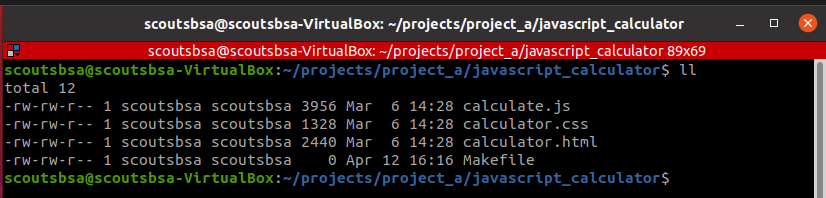
\includegraphics[width=0.8\linewidth]{project_a_files.png}
      \caption{Project A Files}
      \label{fig:project_a_files}
    \end{figure}
    \FloatBarrier

    \textbf{calculator.js} is the \textit{JavaScript} file for the calculator. 
    This file is where you will do all of your work for this project.

    \textbf{calculator.css} is the \textit{Cascading Style Sheets} file for the calculator.
    This file specifies certain things about how the calculator looks such as the colors.
    You are welcome to edit this file to change colors, but not required.

    \textbf{calculator.html} is the \textit{HTML} file which serves as the entry point for this project.
    \textit{HTML} has been the backbone of the internet for decades, so feel free to look into this file, but there is no need to modify it.

    \textbf{Makefile} is a file I have created to help you run this project more easily.
    That being said it is extremely small and simple so feel free to look into it.

    Now that you know what files are in the folder let's do some programming!
    %If you find yourself wondering what something means \autoref{app:programming_basics}
    To start VSCode run \texttt{code . \&}.
    Once VSCode is open click the \textit{calculate.js} file on the left-hand side.

  \section{ToDo 1 - Creating a Variable}
  \label{sec:project_a_todo_1}

    Throughout this code you will see 4 comments which contain ToDo's.
    I would recommend working through them in the order provided.

    To start run the calculator using \texttt{make}.
    This will open a browser window (like the one in \autoref{fig:project_a_todo_1_browser}).
    When you hit a number you should see a message in the console (bottom of the screen telling you which number is pressed).
    
    Now try pressing '+'.
    What do you see in the console?
    If you haven't hit the \textit{clear} button yet then you should see a message followed by an error that says
      \texttt{operator is not defined}.
    
    \begin{figure}[ht]
      \centering
      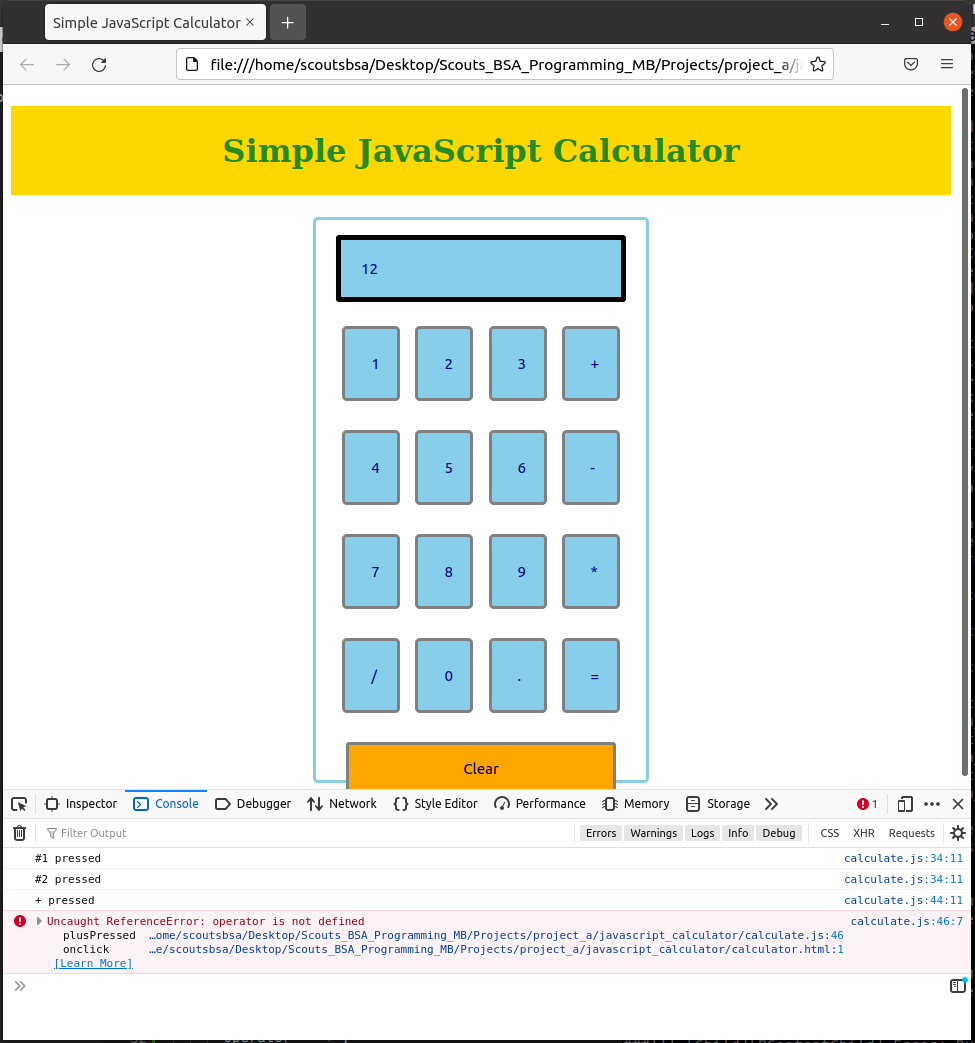
\includegraphics[width=0.8\linewidth]{project_a_todo_1_browser.png}
      \caption{Project A Files}
      \label{fig:project_a_todo_1_browser}
    \end{figure}
    \FloatBarrier

    So let's fix this.
    Find the comment which contains the ToDo 1 task '\textit{Create a variable called 'operator' to represent the last operator clicked}'.
    The two lines above the comment declare other variables.
    Can you figure out how to create the new one?

    Once you think you've got it try running \texttt{make} again.
    You shouldn't see the same error and all the numbers should work.
    Additionally, '+', '=', and clear should work for addition.

  \section{ToDo 2 - Variable Assignment and Display}
  \label{sec:project_a_todo_2}
  
    Once you've got addition working let's get subtraction going.
    Find ToDo \#2 in the \texttt{minusPressed} function.

    For this part of the task we are doing two things:
    
    \begin{enumerate}
      \item Set the previous value variable to the current value
      \item Display the current value
    \end{enumerate}

    This was done in the \texttt{plusPressed} function.
    Can you use it to perform this task?

    Once you've worked through this ToDo, run \texttt{make} again.
    Now addition and subtraction should both be working!

  \section{ToDo 3 - Add Multiplication Functionality}
  \label{sec:project_a_todo_3}

    This next step should enable multiplication to work correctly.
    Find the \texttt{calculate} function and ToDo \#3 inside.
    This task is to add capability for the calculate function to handle multiplication and division.

    Again this function already contains how it is done for addition and subtraction.
    How do you think it is done for multiplication and division?

    Once you've gotten it done try multiplying with the calculator.
    Be ready to explain why changing this function seems to change how the \texttt{timesPressed} function works.

  \section{ToDo 4 - Add Division Functionality}
  \label{sec:project_a_todo_4}

    This final step is the most complex.
    Use everything you've learned so far to create a function called dividePressed which performs division.
    Once this is working you are done with Project A!

    Discuss the findings from this project with your councilor.